% Created 2023-01-30 lun. 04:03
% Intended LaTeX compiler: pdflatex
\documentclass[letterpaper]{article}
\usepackage[utf8]{inputenc}
\usepackage{lmodern}
\usepackage[T1]{fontenc}
\usepackage[top=1in, bottom=1.in, left=1in, right=1in]{geometry}
\usepackage{graphicx}
\usepackage{longtable}
\usepackage{float}
\usepackage{wrapfig}
\usepackage{rotating}
\usepackage[normalem]{ulem}
\usepackage{amsmath}
\usepackage{textcomp}
\usepackage{marvosym}
\usepackage{wasysym}
\usepackage{amssymb}
\usepackage{amsmath}
\usepackage[theorems, skins]{tcolorbox}
\usepackage[version=3]{mhchem}
\usepackage[numbers,super,sort&compress]{natbib}
\usepackage{natmove}
\usepackage{url}
\usepackage[cache=false]{minted}
\usepackage[strings]{underscore}
\usepackage[linktocpage,pdfstartview=FitH,colorlinks,
linkcolor=blue,anchorcolor=blue,
citecolor=blue,filecolor=blue,menucolor=blue,urlcolor=blue]{hyperref}
\usepackage{attachfile}
\usepackage{setspace}
\author{Thomas Lebrat}
\date{\textit{<2023-01-29 dim.>}}
\title{RADIOSONDAGE}
\begin{document}


\section{Le ballon sonde}
\label{sec:org6aaa7c0}

\textbf{\textbf{Le radio-sondage}} est une technique de mesure en altitude des propriétés de l'atmosphère par ballon sonde. Des capteurs mesurent les variations de 3 paramètres en fonction de l'altitude : 

\begin{table}[htbp]
\label{name}
\centering
\begin{tabular}{|c|c|c|c|}
altiude & pression & température & humidité\\
\hline
z(km) & P(Pa) & T(K) & q(g.m\textsuperscript{-3})\\
\ldots{} & \ldots{} & \ldots{} & \ldots{}\\
\end{tabular}
\end{table}


\textbf{\textbf{Le principe est simple !}} On rempli un ballon d’un gaz plus léger que l’air afin de lui communiquer une poussée verticale : il s’élève, en pratique à une vitesse de l’ordre de quelques mètres par seconde, jusqu'à ce que la dilatation du gaz contenu dans son enveloppe ne provoque son éclatement, généralement observé vers 20 à 30 kilomètres d'altitude.

\bigskip


\bigskip

\textbf{\textbf{Remarques}} :

\begin{itemize}
\item La plateforme est équipée d'un parachute qui permettra après éclatement du ballon de récupérer le materiel. Vous pouvez consulter sur ce site les trajets : \url{https://sondehub.org}
\end{itemize}


\begin{itemize}
\item L'instrument permet en outre de mesurer les directions du vent grâce à un suivi de la trajectoire du ballon. Ce point ne sera pas abordé aujourd'hui (un possible sujet d'exposé).

\item Les données une fois récoltées sont reportées sur des diagrammes thermodynamiques qui permettent d'étudier la stabilité des masses d'air \emph{in situ} (voir exercice papier 2 pour approfondissement)
\end{itemize}

\bigskip

\textbf{\textbf{Travail à réaliser}} : Partant de l'observation que dans la troposphère (voir structure de l’atmosphère, J.Vidot), la température décroît linéairement suivant un taux proche de  \(a = 6.5~K.km^{-1}\), proposer une explication au mécanisme contrôlant l'ascension du ballon sonde jusqu'à son éclatement.

\bigskip

\textbf{\textbf{Notations}} : la température au sol est notée \(T_0\). Le ballon sonde sphérique de rayon \(r\), fermé et placé dans l’air, contient une masse \(m\) d’hélium. Les accessoires et l'enveloppe ont une masse légèrement inférieure au kilogramme (\(m_{0} = 750 g\)).
On rappelle la valeur de la constante des gaz parfaits, \(R = 8.31 ~J.K^{-1}.mol^{-1}\).

\bigskip

\textbf{\textbf{Schéma}} : \ldots{}


\newpage

\subsection{Force ascensionnelle}
\label{sec:org6f8fd14}

Discutons les points suivants avant de modéliser le système : 

\begin{itemize}
\item définition de la force ascensionnelle : résultante à l'altitude nulle des forces extérieures exercées sur l'ensemble du système étudié (ballon + gaz).

\item accélération de pesanteur : prendre une valeur approchée à une décimale est-il suffisant ? [une discussion au sujet de la valeur de \(g\) sur le globe est engagée].

\item C.I : le ballon est gonflé au sol de sorte qu’à la température \(T_0\) et pour une pression extérieure de \(P_{0} = 1 ~bar\), le rayon \(r_{0}\) soit de \(75 ~cm\).
\end{itemize}

\textbf{\textbf{Questions simples pour s'échauffer:}}

\begin{enumerate}
\item Estimer la masse volumique de l'air \(\rho_0\)
\item Estimer la masse de gaz hélium à injecter.
\item Proposer une expression de la force permettant l'ascension du ballon en fonction des paramètres  \(r_0\),\(m_0\), \(m\), \(g\) et \({\rho}_0\). On pourra partir des premiers principes de la mécanique ou faire un raisonnement sur les dimensions des grandeurs considérées.
\item Quelle est la valeur maximale de la masse des accessoires et de l’enveloppe que peut supporter un tel ballon  ?
\end{enumerate}

\subsection{Pression atmosphérique (un soupçon de thermo)}
\label{sec:org9432046}

\begin{itemize}
\item loi de nivellement
\end{itemize}
Montrer que la pression atmosphérique \(P(z)\) à l’altitude \(z\) peut s’écrire en fonction de la température \(T(z)\) sous la forme 


$$ P(z) = P_0 \left( \frac{T(z)}{T_0} \right)^{\eta} $$

où \(\eta\)  est une constante que l’on exprimera en fonction de \(M_a\) (masse molaire de l’air), \(g\), \(a\) et \(R\).


\begin{itemize}
\item Etude sommaire des variations de pression
\end{itemize}

On donne \(\eta=5.26\). Estimer la valeur de la pression à différents altitudes (par ex les tous les kilomètres jusqu'à 5 km)

\begin{table}[htbp]
\label{pression}
\centering
\begin{tabular}{|c|c|c|c|c|c|c|}
z(km) & 1 & 2 & 3 & 4 & 5\\
\hline
P(Pa) & \ldots{} & \ldots{} & \ldots{} & \ldots{}. & \ldots{}\\
\end{tabular}
\end{table}


\subsection{Altitude maximale (une pincée de méca)}
\label{sec:orge7c0935}

En négligeant la résistance élastique du ballon, on pourra considérer que l’hélium est
à la pression atmosphérique.


\begin{itemize}
\item Déterminer l'expression de la force ascensionnelle \(F\) pour une altitude \(z\) fixée
\item La ballon ne peut pas se dilater au delà de 2 mètres. Calculer un ordre de grandeur de l'altitude atteinte par le ballon avant son éclatement.
\end{itemize}








\newpage



\section{Formation d'un nuage}
\label{sec:orgb0553e2}


Les phénomènes météos - souvent complexes et parfois spectaculaires dans leurs manifestations - ont des origines variées et une compréhension fine nécessite de prendre en compte de nombreux paramètres ! Pour autant un phénomènes assez banal est expliquable facilement car uniquement du au déplacement adiabatique de masses d’air. Cet exercice se propose d’expliquer qualitativement la création d’un courant ascendant  pouvant conduire à la formation d'un nuage.

On discutera (éventuellement) la pertinence des hypothèse suivantes sur l'air atmosphérique : (H1) air sec ou air humide, (H2) gaz parfait, (H3) capacités thermiques massiques constantes, (H4) pesanteur constante.

Un point de l'atmosphère est repéré par ses coordonnées cartésiennes dans un trièdre orthonormé (Oxyz), tel que l'axe (Oz) coïncide avec la verticale ascendante, la cote z étant prise au niveau de la mer.


\subsection{En l'abscence de mouvement (équilibre)}
\label{sec:org6426722}

Des relevés expérimentaux montrent qu'en l'absence de mouvement des masses d'air, la température est fonction de l'altitude \(z\) suivant une loi affine : 

$$ T(z) = T_{0} - \lambda z $$

On peut montrer que \(P\) et \(T\) à l'altitude \(z\) sont liées par la relation suivante, appelée loi de nivellement barométrique:

$$ T =T_0 \left( \frac{P}{P_0}  \right)^{q} $$

S'il vous reste quelques souvenirs de thermo vous pouvez essayer de retrouver cette relation. Déterminer l’exposant \(q\) en fonction de \(M\), \(g_0\), \(\lamdda\) et \(R\) et faites l'application numérique pour une valeur convenablement choisie de \(\lambda\).




\subsection{Apparition d'un mouvement (instabilté)}
\label{sec:org3d0ae25}

L'état d'équilibre précédent est réalisé lorsque les isothermes (niveaux où T=Cte) et les isobares (P=Cte) coïncident avec les équipotentielles du champ de pesanteur c-à-d les surfaces d'équation \(z = cte\). (pour les curieux/ses voir fluides barotrope/baroclines \ldots{}). En présence d’hétérogénéités au niveau du sol, comme des écarts de température d'un point à un autre, l'air s'échauffe différemment et peut se mettre en mouvement.

\bigskip

\begin{figure}[htbp]
\centering
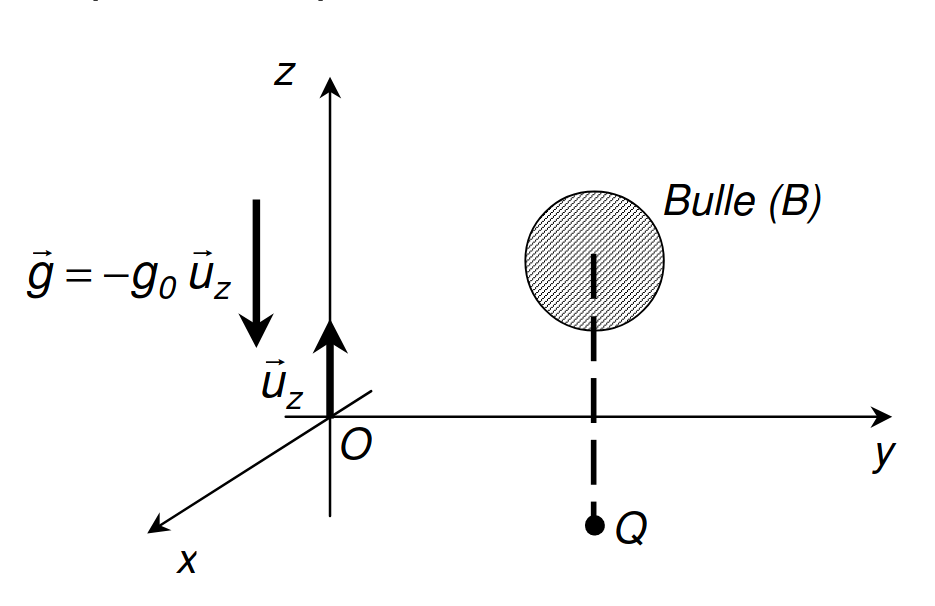
\includegraphics[width=.9\linewidth]{./Ex2a.png}
\end{figure}


On se place à l'altitude z et à la verticale du point Q et on suppose que l'air est localement, plus chaud que l'air avoisinant. Tout se passe comme si une poche de gaz était limitée par une enveloppe souple et non tendue. La bulle de gaz évolue sans échanger de matière ni de chaleur avec l'extérieur. La pression de la bulle restant égale à celle de l'air environnant à la même altitude. On supposera que la température de l'air environnant reste toujours fonction affine de la température.

\begin{enumerate}
\item On note \(P_B\), \(T_B\) et \(\rho_B\) la pression, la température et la masse volumique du gaz emprisonné dans la bulle ; \(T_A\) et \(\rho_A\) la température et la masse volumique de l'air environnant à la même altitude. Montrer que la bulle s'élève si \(T_B > T_A\).

\item Le gaz emprisonné dans la bulle subit donc une transformation adiabatique que l'on supposera réversible. On appelle \(T_1\) la température du gaz dans la bulle à l'altitude de sa formation \(z_1\) et \(P_1\) la pression correspondante. Exprimer \(T_B\) en fonction de \(T_1\), \(P_1\) et \(P_B\).

\item Montrer qu'il existe une altitude plafond \(z_2\) pour l'ascension de la bulle. On note \(T_2\) et \(P_2\) la température et la pression de la bulle lorsqu'elle arrive à cette altitude. Calculer numériquement \(T_2\) et \(P_2\) pour \(T_1 = 280 K\) et \(z_1 = 2 km\). En déduire la valeur de l'altitude plafond \(z_2\) à laquelle se stabilise la bulle.4.

\item L'air étant supposé maintenant humide (mélange d'air sec et de vapeur d'eau), montrer comment l'on pourrait expliquer qualitativement la possibilité de formation d'un nuage au cours de l'ascension de cette bulle.
\end{enumerate}


\newpage

\section{Quelques références}
\label{sec:org5a0fb81}


Les sites suivants ont été consultés pour préparer cette activité : 

\begin{itemize}
\item \url{https://labolycee.org/mecanique-du-vol-dun-ballon-sonde}

\item \url{http://www.msc.univ-paris-diderot.fr/\~phyexp/pmwiki.php/Convention/ConvectionEtPanacheThermique}

\item \url{https://web.archive.org/web/20081119164748/http://www.meteofrance.com/FR/glossaire/designation/693\_initie\_view.jsp}

\item \url{http://b.louchart.free.fr/Concours\_et\_examens/Centrale\_Supelec/Sujets/2008\_TSI\_Physique\_1.html}

\item \url{https://planet-terre.ens-lyon.fr/ressource/mouvts-enveloppes-fluides2.xml}
\end{itemize}
\end{document}
